\Chapter{A lekérdezőnyelv}

\section{Alaptípusok}

A lekérdezőnyelv típusos. Tartalmaz előre definiált típusokat (\textit{alaptípusok}, \textit{gyári típusok}), illetve a nyelv lehetőséget ad új típusok definiálására is (\textit{felhasználói típusok}).

Az alaptípusok hierarchiáját \aref{fig:types} ábrán láthatjuk. Az élek itt tartalmazási kapcsolatot jelölnek. A nyelv csak kompozícióra ad lehetőséget.

A típusokból hasonlóképpen tudunk példányokat létrehozni, mint ahogy az objektum orientált programozási nyelvekben. A típus nevét követő zárójelekben adhatjuk meg a példány létrehozásához szükséges értékeket egy vesszővel elválasztott listában.

Minden objektumnak a típusa mellett van azonosítója is. Ezt az \texttt{id} attribútumában tárolja. Értéket példányosításkor automatikusan kap. Az objektumtól le tudjuk azt kérdezni, viszont változtatni nem lehet.

A következő szakaszokban az alaptípusok bemutatására kerül sor. A használati módjuk, paraméterezésük szemléltetéséhez már itt is lekérdezések szerepelnek, viszont azok részletes bemutatása majd csak a műveleti rész taglalásánál szerepel.

\begin{figure}[htb]
\begin{center}
    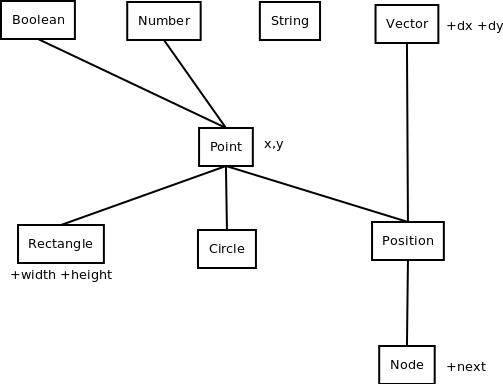
\includegraphics[scale=0.5]{images/types}
    \caption{A lekérdezőnyelv alaptípusai}
    \label{fig:types}
\end{center}
\end{figure}

\begin{comment}{A képet majd szépíteni kellene még kicsit. A négyzetrácsnak és a kék pontoknak nem kelllene látszódnia. (DIA-ban van külön export funkció ehhez.)}
\end{comment}

\subsection{Boolean}

A \textit{Boolean} a nyelvben a logikai adattípus. Értéke \texttt{true} vagy \texttt{false} lehet. Paraméter nélküli létrehozás esetén az alapértelmezett értéke \texttt{false}. Az alábbi példákban az \texttt{azeroth} nevű térképre kerülnek beszúrásra logikai értékek.

\begin{sql}
INSERT Boolean() INTO azeroth;
INSERT Boolean(true) INTO azeroth; 
INSERT Boolean(false) INTO azeroth;
INSERT Boolean(
    SELECT bool FROM azeroth
    WHERE bool IS Boolean AND bool.id = "bool11"
) INTO azeroth;
\end{sql}

Az utolsó példából látható, hogy a logikai típusú objektum is teljes értékű objektum, így az is rendelkezik azonosítóval (\texttt{id}).

\subsection{Number}

A \textit{Number} típus valós vagy egész szám 4 byteon való tárolására alkalmas. A lekérdezőnyelv nem különböztet meg előjeles és előjel nélküli változatot.

\begin{sql}
INSERT Number(1.2) INTO azeroth;
INSERT Number(12) INTO azeroth;
INSERT Number(
    SELECT number FROM azeroth
    WHERE number IS Number AND number.id = "numberasd11"
) INTO azeroth;
INSERT Number(
    SELECT number FROM azeroth
    WHERE number HAS x AND number.x IS Number AND number.id = "num11"
) INTO azeroth;
\end{sql}

\subsection{String}

Szöveges értékek tárolására a \textit{String} típust használhatjuk.

\begin{sql}
INSERT String("alma") INTO azeroth;
INSERT String(
    SELECT string FROM azeroth
    WHERE string IS String AND string.id = "stringasd11"
)
INTO azeroth;
\end{sql}

\subsection{Point}

A térképen az elemek helyét pontok adják, amelyet \textit{Point} típusú objektumokban tárolhatunk. A pontnak sem kiterjedése, sem iránya nincs. Tulajdonképpen két \textit{Number} típusú értéket fog össze egy egységbe. A pont koordinátáit a geometriában használatos $(x, y)$ párral adhatjuk meg.

\begin{sql}
INSERT Point(10, 20) INTO azeroth;
INSERT Point(Number(10), Number(20)) INTO azeroth;
INSERT Point(Number(10), 20) INTO azeroth;
INSERT Point(10, Number(20)) INTO azeroth;
INSERT Point(Point(10, 10)) INTO azeroth;
INSERT Point(
    SELECT point FROM azeroth
    WHERE point IS Point AND point.id = "pointasd11"
) INTO azeroth;
\end{sql}

Az utolsó beszúrás esetében egy másik \textit{Point} típusú objektumra hivatkozunk. Amennyiben annak az értéke változik valamelyik a kettő közül, akkor ennek is változni fog.

\begin{sql}
INSERT Point(
    SELECT number FROM azeroth
    WHERE number is Number AND number.id = "numasd11", 10
) INTO azeroth;
\end{sql}

Ilyenkor a pont \texttt{x} attribútuma egy másik \textit{Number} típusú objektumra mutat, tehát ha az változik, akkor a pont attribútuma is fog.

\begin{sql}
INSERT Point(
    SELECT number FROM azeroth
    WHERE number is Number AND number.id = "numasd11",
    SELECT number FROM azeroth
    WHERE number is Number AND number.id = "numasd12"
) INTO azeroth;
\end{sql}

Ebben mind a két attribútuma más \textit{Number} objektumra mutat.

\subsection{Vector}

A \textit{Vector} típus itt a geometriai értelemben véve irány tárolását teszi lehetővé. A ponthoz hasonlóan ez is két \textit{Number} értéket fog össze, ennek viszont csak iránya van, helye nincsen.

\begin{sql}
INSERT Vector(10, 20) INTO azeroth;
INSERT Vector(Number(10), Number(20)) INTO azeroth;
INSERT Vector(Number(10), 20) INTO azeroth;
INSERT Vector(10, Number(20)) INTO azeroth;
INSERT Vector(Vector(10, 20)) INTO azeroth;
INSERT Vector(
    SELECT vector FROM azeroth
    WHERE vector IS Vector AND vector.id = "vetorasd11"
) INTO azeroth;
\end{sql}

Ilyenkor egy másik \textit{Vector} objektumra hivatkozik, tehát ha annak az értéke változik valamelyik a kettő közül, akkor ennek is fog.

\begin{sql}
INSERT Vector(
    SELECT number FROM azeroth
    WHERE number is Number AND number.id = "numasd11", 10
) INTO azeroth;
\end{sql}

Ilyenkor a vector \texttt{dx} attribútuma egy másik \textit{Number} objektumra mutat, tehát ha az változik, akkor ez is fog.

\begin{sql}
INSERT Vector(
    SELECT number FROM azeroth
    WHERE number is Number AND number.id = "numasd11",
    SELECT number FROM azeroth
    WHERE number is Number AND number.id = "numasd12"
) INTO azeroth;
\end{sql}

A ponthoz hasonlóan itt is megadható függetlenül a két \textit{Number} érték.

\subsection{Dimension}

Egy szélesség és egy magasság értéket tárol. Mindkettő típusa \textit{Number}.

\begin{sql}
INSERT Dimension(10, 20) INTO azeroth;
INSERT Dimension(Number(10), Number(20)) INTO azeroth;
INSERT Dimension(Number(10), 20) INTO azeroth;
INSERT Dimension(10, Number(20)) INTO azeroth;
INSERT Dimension(Dimension(10,10)) INTO azeroth;
INSERT Dimension(
    SELECT dimension FROM azeroth
    WHERE dimension IS Dimension AND dimension.id="dimensionasd11"
) INTO azeroth;
\end{sql}

Az utóbbi esetben egy másik Dimension objektumra hivatkozik, tehát ha annak az értéke változik valamelyik a kettő közül, akkor ennek is fog. Hasonlóan kezelhetjük az egyes esetek külön-külön hivatkozásokkal való megadását is, mint ahogy a pont és a vektor esetében.

\begin{sql}
INSERT Dimension(
    SELECT number FROM azeroth
    WHERE number is Number AND number.id = "numasd11", 10
) INTO azeroth;
INSERT Dimension(
    SELECT number FROM azeroth
    WHERE number is Number AND number.id = "numasd11",
    SELECT number FROM azeroth
    WHERE number is Number AND number.id = "numasd12"
) INTO azeroth;
\end{sql}

Az utolsóban szintén itt is mind a két attribútuma más \textit{Number} típusú objektumra mutat.

\subsection{Rectangle}

A \textit{Rectangle} típus téglalap adatainak tárolására szolgál. Tartalmaz egy pontot, amelyben tárolja a bal felső sarkának koordinátáit, illetve egy kiterjedést, amely a szélesség és magasság attribútumokat adja.

\begin{sql}
INSERT Rectangle(Point(10,10), Dimension(100, 200)) INTO azeroth;
INSERT Rectangle(Rectangle(10, 10, 100, 100)) INTO azeroth;
\end{sql}

Itt az a lényeg, hogy lehet belül azzal a new nélküli kifejezéssel is visszaadatni új objektumot.

\begin{sql}
INSERT Rectangle(10, 10, 100, 200) INTO azeroth;
INSERT Rectangle(10, 10, Dimension(100, 200)) INTO azeroth;
INSERT Rectangle(Point(10, 10), 100, 200) INTO azeroth;
INSERT Rectangle(
    SELECT rectangle FROM azeroth
    WHERE rectangle IS Rectangle AND id = "rectasd11"
) INTO azeroth;
INSERT Rectangle(
    SELECT number FROM azeroth
    WHERE number is Number AND number.id = "numasd11",
    SELECT number FROM azeroth
    WHERE number is Number AND number.id = "numasd12",
    SELECT number FROM azeroth
    WHERE number is Number AND number.id = "numasd13",
    SELECT number FROM azeroth
    WHERE number is Number AND number.id = "numasd14"
) INTO azeroth;
\end{sql}

Itt mind a 4 paraméter egy lekérdezés eredménye, azaz mind mutat egy másik objektumra.
Attól függetlenül, hogy hozzuk létre a téglalapot, ezeket egy pont és egy kiterjedés objektumban fogja tárolni.

\subsection{Circle}

\begin{comment}{Még egyeztetés alatt a létjogosultsága.}
\end{comment}

\subsection{Position}

A pozíciók leírásához használhatjuk a \textit{Position} osztályt. Ennek van helye és iránya. Lényegében egy pont és egy vektor objektumot fog össze egy logikai egységbe.

\begin{sql}
INSERT Position(Point(10, 10), Vector(100, 100)) INTO azeroth;
INSERT Position(Position(10, 10, 100, 100)) INTO azeroth;
\end{sql}

A pozíciókat közvetlenül az attribútumok értékeivel, vagy pedig részlegesen a részobjektumaival is példányosíthatjuk.

\begin{sql}
INSERT Position(10, 10, 100, 200) INTO azeroth;
\end{sql}

Ebben az esetben a sorrend \texttt{x}, \texttt{y}, \texttt{dx} és \texttt{dy}. 

\begin{sql}
INSERT Position(10, 10, Vector(100, 200)) INTO azeroth;
INSERT Position(Point(10, 10), 100, 200) INTO azeroth;
INSERT Position(
    SELECT position FROM azeroth
    WHERE position IS Position AND id = "posasd11"
) INTO azeroth;
INSERT Rectangle(
    SELECT number FROM azeroth
    WHERE number is Number AND number.id = "numasd11",
    SELECT number FROM azeroth
    WHERE number is Number AND number.id = "numasd12",
    SELECT number FROM azeroth
    WHERE number is Number AND number.id = "numasd13",
    SELECT number FROM azeroth
    WHERE number is Number AND number.id = "numasd14"
) INTO azeroth;
\end{sql}

Ezekben is, az előzőekhez hasonlóan objektum hivatkozások jönnek létre a példányosítás során.

\subsection{Node}

A nyelv a dinamikus adatszerkezetek leírását láncolással oldja meg. Az alkalmazási területeket figyelembe véve általában pozíciók láncolására lehet szükség. A \textit{Node} típus egy pozíció típusú attribútumot és egy hivatkozást tartalmaz a következő \textit{Node} objektumra. Ennek a segítségével megadhatunk útvonalakat, fákat vagy általános irányított gráfokat.

\begin{sql}
INSERT Node(Node(10, 10, 100, 100, NULL)) INTO azeroth;
\end{sql}

A csomópontnak ekkor a pozícióra jellemző attribútumait egészítjük ki egy referenciával. A \texttt{NULL} ez esetben a sehova sem mutató, érvénytelen referenciát jelenti.

\begin{comment}{Egységesen kellene a true, false-al!}
\end{comment}

\begin{sql}
INSERT Node(10, 10, 100, 100, NULL) INTO azeroth;
INSERT Node(10, 10, 100, 100,
    SELECT node FROM azeroth
    WHERE node IS Node AND node.id = "nodeasd11"
) INTO azeroth;
\end{sql}

Itt már úgy hozunk létre egy csomópontot, hogy az egy másik, már létező csomópontra mutat.

\begin{sql}
INSERT Node(10, 10, 100, 100, Node(200, 200, 2000, 2000, NULL)) INTO azeroth;
\end{sql}

A nyelv ezt a megoldást is lehetővé teszi. Ilyenkor a belső csomópont objektumra fog mutatni, ami viszont ilyenkor még nincs a térképen, de ez így egyúttal létre is hozza, hogy ő hivatkozik rá a láncban.

\begin{sql}
INSERT Node(10, 10, 100, 100, NULL, true) INTO azeroth;
\end{sql}

Ha az 5. paraméternek egy \texttt{true} értéket adunk meg, akkor az azt jelenti, hogy ez egy Lánc első eleme, innen indul ki az összes többi. (Amennyiben az utolsó elem erre mutat, akkor kapunk egy körutat.)

\begin{sql}
INSERT Node(10,10, 100, 100, NULL, false) INTO azeroth;
\end{sql}

Így is létrehozható egy csomópont. Ez az alapértelmezett eset, tehát ha nem tüntetjük fel, hogy az utolsó paraméter értéke \texttt{false}, akkor alapértelmezés szerint ugyanezt kapjuk.

\begin{comment}{Ennek az utolsó paraméternek majd még utána kell gondolni!}
\end{comment}

\begin{sql}
INSERT Node(10,10, 100, 100) INTO azeroth;
\end{sql}
Ha elhagyjuk azt a paramétert, ami a következő csomópontra mutatna, akkor azzal sincs semmi gond, mert az automatikusan beilleszti oda a NULL értéket.

\subsection{Path}

A \textit{Path}, útvonal típus csomópontok halmazát tárolja.

\begin{sql}
INSERT Path(
    Node(10,10,10,10),
    Node(10,20),
    Node(10,10,100,35)
) INTO azeroth;
\end{sql}

Itt az útvonal úgy jön létre, hogy a paraméterlistában szereplő csomópontokat úgy hozza létre, hogy paraméterlistában való elhelyezkedés szerint adja értékül a \texttt{next} értéknek mindig a következőt. Az utolsó elem \texttt{next} attribútuma \texttt{NULL} értéket kap.

Minden csomópont objektumnak van egy \texttt{isFirst} logikai típusú attribútuma, ami csak az első elemnek vesz fel igaz értéket, hogy tudjuk honnan indul az útvonal. Ez az \texttt{isFirst} az útvonal létrehozási mechanizmusban automatikusan kap értéket, erről a felhasználónak nem kell gondoskodnia.

Látható, hogy az egyik csomópontot kevesebb (mindössze kettő paraméterrel) hoztuk létre. Ez nem jelent semmi problémát, ilyenkor az irány nincs megadva, de arra nem is feltétlenül van szükség.

A \textit{Node} adattípus leírásánál elmondtuk, hogy a \texttt{Node(10, 10, 10, 10)} hívással nem adjuk meg a következő Nodera mutató elemet, így az autómatikusan NULL lesz. Amennyiben ez  \textit{Path} inicializálásnál történik, akkor a következő csomópont hivatkozását kapja meg (amennyiben nem az utolsó helyen szerepel a paraméter).

\begin{sql}
INSERT Path(
    SELECT node FROM azeroth
    WHERE node IS Node AND node.id = "nodeasd11"
) INTO azeroth;
\end{sql}

Egy útvonal nem hozható létre a meglévő csomópontok összegyűjtéséből. Az útvonal inicializálásnál nem szerepelhet egyetlen szelekciós utasítás sem, mert az hibákhoz vezetne.

Egy objektum ha referenciát tartalmaz egy másik objektumra akkor az eléri bármikor a hivatkozottat, viszont a hivatkozott nem tud hivatkozni arra aki rá hivatkozik. Erre nincs nyelvi elem definiálva, hisz a gyakorlatban ritkán van erre szükség, kevés esetben lenne alkalmazható, így kimaradt a lekérdező nyelv eszközkészletéből.

\section{Támogatott operátorok}
\begin{itemize}
\item = 
\item <= 
\item >= 
\item > 
\item < 
\item <> (nem egyenlő) 
\item OR 
\item AND 
\item IS 
\item COLLIDE
\item NOT
\end{itemize}

A fenti operátorok boolean értékkel térnek vissza.

Lássunk mindegyikre egy példát:
\begin{sql}
SELECT mine FROM azeroth WHERE mine.id = "asd11";
SELECT mine FROM azeroth WHERE mine.x <= 10;
SELECT mine FROM azeroth WHERE mine.y >= 10;
SELECT mine FROM azeroth WHERE mine.x <> 20;
\end{sql}


A mine.x operandus a háttérben egy mine HAS x feltételt is jelent, de ezt nem kell feltüntetnie a felhasználónak. A mine HAS x jelentése, hogy az adott objektumnak van x attribútuma, vagy sem. Sokáig nyelvi szinten megtalálható volt a HAS operátor, viszont a kényelmi szempontok miatt ezt automatikusan kezeli az adatbázismotor.
 
\begin{sql}
SELECT mine FROM azeroth WHERE mine.stone.location.x > 10;
\end{sql}

A fent látható lekérdezés olyan objektumokat kérdez le, amelyeknek van stone attribútuma, aminek van location attribútuma, aminek van x attribútuma(ezekre a HAS feltétel kiértékelődik) és ennek az x attribútumnak az értéke nagyobb mint 10.

\begin{sql}
SELECT mine FROM azeroth WHERE mine IS Mine;
\end{sql}

Az IS operátor az objektum típusának ellenőrzésére szolgál, az IS bal oldalán egy szimbólum, jobb oldalán pedig egy Class név kell szerepeljen.

\begin{sql}
SELECT mine FROM azeroth WHERE mine.x = 10 AND mine.y < 20;
\end{sql}

A logikai műveletek a WHERE után kombinálhatóak is természetesen:

\begin{sql}
SELECT mine FROM azeroth WHERE mine.x = 10 AND mine.y = 20 OR mine.id=100;
\end{sql}

Ha nincs zárójelezés, akkor sorban veszi a feltételeket.

\begin{sql}
SELECT mine FROM azeroth WHERE mine.x = 10 AND (mine.y = 20 OR mine.id = 100);
\end{sql}

\begin{sql}
SELECT mine FROM azeroth WHERE mine.x = 10 AND NOT (mine.y = 20 OR mine.id = 100 OR 10=10);
\end{sql}

A fenti lekérdezés azokat az objektumokat gyűjti ki, amelyek x attribútuma 10, és y attribútuma nem egyenlő 20, és az id-jük nem egyenlő 100-al.
\begin{sql}


Az alábbi lekérdezés azokat az objektumokat választja ki, amelyek nem tartalmazzák a 10, 10 pontot.
\begin{sql}
SELECT mine FROM azeroth WHERE NOT(mine COLLIDE POINT(10, 10));
\end{sql}


A kiértékelésben a zárójelnek szerepe lehet, ezt az eszközt a felhasználó kezébe adja az adatbázis.

\section{Saját osztályok definiálása}

\section{Metódusok a lekérdező nyelvben}

Csak a gyárilag definiált osztályok rendelkeznek metódusokkal(Boolean,Number,Vector,Rectangle,stb.).
Ezek gyári szolgáltatások az adott adattípushoz. Viszont amikor a felhasználó készít saját Osztálydefiníciót, ő csak adatleírást végezhet, metódusokat nem definiálhat hozzájuk. A gyárilag elkészített metódusok a típusokhoz valamely szolgáltatást jelentenek. Jelenleg egyetlen metódust definiáltunk a lekérdezőnyelvbe, ami a distanceFrom(Number x, Number x). Ez a metódus visszaad egy Number értéket, ami a távolság az objektum és a megadott pont között. Ezt a metódust minden olyan objektumra meg lehet hívni, amely rendelkezik (x,y) koordinátákkal, illetve szélesség(width), és magasság(height) attribútumokkal.

\section{DDL adatdefiníciós utasítások}

-CREATE: Létrehozó parancs, mellyel objektumokat vagy classokat lehet létrehozni.

Adatbázis létrehozás:
\begin{sql}
CREATE DATABASE db;
\end{sql}

A fenti lekérdezés hatására létrejön egy új adatbázis, "db" névvel. Az adatbázis fogja össze a benne tárolt Mapeket. 

Térkép létrehozás:
\begin{sql}
CREATE MAP azeroth;
\end{sql}
Amikor MAP-et hozunk létre, akkor a megnyitott adatbázison belül egy új térkép jön létre, a lekérdezésben megadott névvel.

Osztálydefiníció létrehozása:
\begin{sql}
CREATE CLASS Mine(
	Number age,
	String name,
	Number x,
	Number y
); 
\end{sql}

Automatikusan minden INSERT lekérdezés hatására beillesztődik egy id attribútum érték az objektumhoz. A definiált classokban van id attribútum, azt nem kell definiálni a CREATE lekérdezésben.

Amikor definiálunk egy osztályt, akkor nincs lehetőségünk öröklődésre, mint például Java nyelven. Tervezéskor a kompozíciót tartottuk a legmegfelelőbb megoldásnak, ami azt jelenti, hogy nem leszármaztatunk egy osztályból, hanem adattagként tároljuk azt, és tovább hívjuk annak metódusait.

Az osztálydefiníciókban természetesen megadhatunk attribútum típusként más osztálydefiníciókat is:

\begin{sql}
CREATE CLASS Mine(
	Stone stone,
	Number size
);

CREATE CLASS Mine(
	Number kor DEAFAULT 18
);
\end{sql}

A DEFAULT integritási feltétel azt jelenti amit SQL nyelvben is, tehát, ha az adott attribútum INSERT lekérdezés hatására nem töltődik fel, akkor a DEFAULT kulcsszó után feltüntetett érték fog automatikusan adódni neki. DEFAULT csak primitív típusú(String, Number, Boolean) attribútumoknál használható.


A MAP-eket és a CLASS-okat is az adatbázis fogja össze.
Amikor létrehozunk egy osztálydefiníciót, akkor azt az adatbázishoz definiáljuk, nem pedig külön a térképekhez, tehát az azonos adatbázisban tárolt térképeken azonos típusú objektumokat tárolhatunk.


Az id-k autómatikus kiosztása úgy történik, hogy minden Map-en külön számláló van erre a célra. Azaz azeroth mapen is van 0 id-jű elem, és og mapen is.A térképek elemei nem keveredhetnek.



-DROP: Elvet egy objektumot vagy osztályt.

\begin{sql}
DROP DATABASE db1;
DROP MAP azeroth;
\end{sql}

A két fenti utasítás értelemszerűen törlést visz végbe. Ha törlök egy adatbázist, akkor minden benne lévő elem törlődik (Class definíciók, Mapek, mentések).
Ha törlök  egy Mapet, akkor minden benne tárolt elem törlődik vele együtt.

\begin{sql}
DROP CLASS Mine;
\end{sql}

Osztálydefiníció megszüntetése. Csak olyan osztálydefiníciót lehet megszüntetni, amire nincs hivatkozás, azaz egyik térképen sincs belőle példány létrehozva.

-ALTER: Szerkezetmódisító művelet. 
Szerkezete módosítani csak az osztálydefinícióknak lehet.Csak azoknál az osztályoknál lehet szerkezetet módosítani, amelyekből egyetlen példány sincs létrehozva az adatbázisban.

Ennek négy típusa van:

Az ADDATTRIBUTE utasítással meglévő osztályhoz adunk hozzá egy újabb attribútumot.
\begin{sql}
ALTER CLASS Mine ADDATTRIBUTE name String;
\end{sql}

A RENAMEATTRIBUTE utasítással egy meglévő attribútumot nevezhetünk át a TO kulcsszó után szereplő értékre.Innentől kezdve ezen a néven lehet rá hivatkozni.
\begin{sql}
ALTER CLASS Mine RENAMEATTRIBUTE size TO name;
\end{sql}

A DELETEATTRIBUTE törli a size attribútumát a Mine osztálydefiníciónak.
\begin{sql}
ALTER CLASS Mine DELETEATTRIBUTE size;
\end{sql}

A RENAMECLASS az osztály nevének megváltoztatása.
\begin{sql}
ALTER CLASS Mine RENAMECLASS BigMine;
\end{sql}


\section{DML adatkezelő utasítások}

-DELETE: Objektum törlés. Objektum alatt a létrehozott Class példányokat értjük.

Az összes Mine típusú elemet kitörli az azeroth térképről.
\begin{sql}
DELETE mine FROM azeroth WHERE  mine IS Mine;
\end{sql}

Minden elemet kitöröl a térképről, aminek "azeroth" a neve.
\begin{sql}
DELETE mine FROM azeroth;
\end{sql}


-UPDATE:
Objektum tartalom módosítás.Az UPDATE is az SQL működésére épül, amikor UPDATE-SET lekérdezésről van szó. Olyankor a WHERE feltételre teljesülő objektumok attribútumainak értékét változtatja meg. Viszont itt térkép adatbázisról lévén szó, az ütközés vizsgálat egyik részét is ezen lekérdezés alatt volt célszerű megvalósítani, ez pedig nem más, mint a csúszós ütközésvizsgálat. Amikor a SET helyett MOVE kulcsszó szerepel a lekérdezésben, olyankor csak az x és y koordinátákat lehet módosítani az objektumoknak, viszont itt a háttérben ütközésvizsgálat történik. 
Tehát amíg a SET kulcsszó hatására biztosan megváltoznak a kijelölt attribútumok értékei(ha léteznek azok az attribútumok), addig MOVE esetén ez nem biztos, hisz ütközés esetén ezt már nem tehetjük meg.Az ütközés vizsgálat ezen részéről a motor implementációs szakaszban fogok bővebben értekezni.



Az azeroth térképen lévő 11 id-jű elem x attribútumának értékét 30-ra állítja ütközésvizsgálat nélkül.
\begin{sql}
UPDATE azeroth SET x = 30 WHERE id="11";
\end{sql}

Az alábbi lekérdezésazt az objektumot mozgatja el, akinek van id tulajdonsága és az "11". Ebben a verzióban a (10,10) pontba toljuk az objektumot, de ez csak akkor, ha nem ütközik egyetlen pályaelemmel sem, aminek solid attribútuma true értéket tárol.
\begin{sql}
UPDATE azeroth MOVE mine TO (10,10) WHERE mine.id = "11";
\end{sql}


-Insert:
Új objektum felvétele egy térképre.A LAYER 1 azt jelenti, hogy a beszúrandó elemek zlayer attribútumát 1-re állítja, a zindexet, pedig az első szinten lévő következő indexre(ezt a háttérben egy vektorban tároljuk, hogy mely layeren mi az aktuálisan kiosztandó zindex szám.)

Az alábbi lekérdezéssel létrehozunk egy új Szobor példányt az azeroth térképre.
\begin{sql}
ADD Szobor(location,name) INTO azeroth VALUES((10,10), "Jani") LAYER 1;
\end{sql}

Az alábbi lekérdezés már az összetettebbek közé tartozik. Szükséges megadni az osztálynév után a attribútumok felépítését, ezzel mondjuk meg, hogy mely atribútumok kapnak értéket a VALUES kulcsszó után felsorolt értékhalmazból.
\begin{sql}
INSERT Mine(x, stone(location(x,y), w, h), age) INTO azeroth VALUES(10,((10, 20), 30, 40), 22);
\end{sql}


Az alábbi lekérdezésnél látható, hogy itt ennek a szobornak egy stone attribútumba egy lekérdezés eredményét adom, ami egy létező objektum, tehát arra fog mutatni(id alapján).
Ha ennek a SELECT lekérdezésnek több értékű halmaz eredménye lesz, akkor hiba dobódik, mivel létrehozásnál egy elemet várunk. Ha üres halmazt kapunk, akkor sem történik meg a beszúrás, akkor is hiba keletkezik.
\begin{sql}
ADD Szobor(x,y,stone(x,y)) INTO azeroth VALUES(10, 10, SELECT stone FROM azeroth WHERE stone IS Stone AND stone.id = "11");
\end{sql}


\section{DQL lekérdező utasítások}


A mine egy kifejezés, amin keresztül elérhetjük az összes  azeroth mapen lévő objektumot. A SELECT után csak egy ilyen kifejezés állhat. Ez azt csinálja, hogy visszaad egy halmazt, amiben minden elem ami a térképen megtalálható(point,rectangle) benne van szűkítés nélkül.
\begin{sql}
SELECT mine From azeroth;
\end{sql}


Az alábbi lekérdezés visszaadja azon elemek halmazát az "azeroth" térképről, melyeknek van x attribútumuk, és azoknak az attribútumoknak a halmazát adná(itt Number típusú x-ek lennének az eredmény halmazban.)
\begin{sql}
SELECT mine.x from azeroth;
\end{sql}


Az alábbi lekérdezésben arra láthatunk példát, amikor a kifejezés több attribútum láncolását tartalmazza. Ekkor Lekérdezi az összes Mine típusú objektum x attribútumát.
\begin{sql}
SELECT mine.stone.location.x FROM azeroth WHERE mine IS Mine;
\end{sql}


- Halmazműveletek a lekérdezésekben:

Két halmaz különbségét az alábbi lekérdezéssel lehetne megoldani(ez a jelenlegi implementációban nincs benne, inkább csak jövőbeli terv).
\begin{sql}
Select mine from azeroth where mine.x < 100 Difference Select mine from azeroth where mine.y > 10; 
\end{sql}

A fenti lekérdezés csak egy terv, viszont az adatbázismotorban ettől függetlenül meglehet valósítani a két halmaz különbségét megvalósító lekérdezést, méghozzá logikai operátorral.

\begin{sql}
Select mine from azeroth where (mine.x < 100 AND NOT mine.y > 10); 
\end{sql}

Két halmaz metszete a következő lekérdezéssel lenne megoldható a tervek szerint:
\begin{sql}
Select mine from azeroth where mine.x < 100 Cutaway Select mine from azeroth where mine.y > 10 Cutaway Select mine From azeroth where mine IS Mine;
\end{sql}
Itt látható, hogy két alkalommal is szerepel a halmazművelet kulcsszava.Ilyenkor sorrendben végrehajtja, azaz először kivonja az első két halmazt egymásból, majd annak eredményéből kivonja az utolsó halmazt.
Könnyű belátni, hogy ez a  halmazművelet is helyettesíthető logikai kifejezésekkel.


Az alábbi lekérdezés teljesen ekvivalens a fenti lekérdezésekkel, melyekben két AlSELECT lekérdezés van, ugyanis azokat az elemeket rakjuk a halmazba melyek x attribútuma 100-nál kisebb, viszont y kisebb mint 10, ez felcserélődik.
\begin{sql}
Select mine from azeroth where mine.x < 100 AND mine.y <= 10;
\end{sql}


Két halmaz Uniójára sincs definiált kulcsszó vagy metódus jelenleg az adatbázismotorba implementálva, viszont logikai operátorokkal ez a funkció is megvalósítható:
\begin{sql}
Select mine from azeroth where mine.x < 100 OR mine.y <= 10;
\end{sql}


Az alábbi két lekérdezés közötti különbség:
\begin{sql}
Select mine.x From azeroth; 
\end{sql}
Ez visszaadja az összes x attribútumot ami a pályán található
\begin{sql}
Select mine From azeroth Where mine HAS x;
\end{sql}
Ez visszaadja az összes Mine típusú elemet, aminek van x attribútuma.


Az alábbi lekérdezés eredménye egy olyan halmaz, amelyben olyan Mine típusú objektumok vannak(maximum 5 darab), amelyek tartalmazzák a 10,10 pontot, majd rendezi mine.id szerint és azután választ ki 5 darabot legfeljebb.
\begin{sql}
SELECT mine
FROM azeroth
WHERE mine COLLIDE [10, 10] AND mine IS Mine
ORDER BY mine.id
LIMIT 5;
\end{sql}


Az alábbi lekérdezés kiválasztja azokat az elemeket a térképről, amelyek tartalmazzák a (10,10) pontot, és a (20,20) ponttól 30 ponttól nagyobb távolságra vannak.
\begin{sql}
SELECT mine
FROM azeroth
WHERE mine COLLIDE [10, 10] AND mine.distanceFrom(20, 20) > 30;
\end{sql}

Kifejezések helyén állhat select, és a selecten belül is használhatunk alSelecteket.
\begin{sql}
SELECT mine
FROM azeroth
WHERE mine COLLIDE[SELECT number FROM azertoth WHERE number.id='21', SELECT number FROM azeroth WHERE number.id='34']
 AND mine.distanceFrom(Point(SELECT number FROM azeroth WHERE number.id='34', SELECT number FROM azeroth WHERE number.id='34')) > SELECT number FROM (SELECT number FROM outland) WHERE number.id='34';
\end{sql}


Az alábbi lekérdezésben rendezzük az elemeket x szerint(itt csak azokat veszi bele, aminek van x attribútuma, majd a rendezett elemből visszaadja az utolsót, ami itt növekvő sorrend miatt a legnagyobb elem lesz.)
\begin{sql}
SELECT mine FROM azeroth ORDER BY mine.x LIMIT 1;
(SELECT mine FROM azeroth ORDER BY mine.x ASC LIMIT 1;)
\end{sql}

ORDER BY esetén az ASC az alapértelmezett beállítás, tehát ha azt nem írjuk ki, akkor is úgy fog lefutni a lekérdezés.

\begin{sql}
SELECT mine FROM azeroth ORDER BY mine.x DESC LIMIT 1;
\end{sql}


ORDER BY használata: Ha x attribútum szerint szeretnénk rendezni az eredményhalmazt, de az eredményhalmazban vannak olyan elemek, melyeknek nincs x attribútuma nincs semmi baj, a lista elejére rakja a rendezett x attribútummal rendelkező elemeket, majd a végére a maradék x attribútummal nem rendelkező elemeket. Ez a rugalmasság miatt lett így implementálva.


\section{Lekérdezések}

\subsection{Ütközésvizsgálat}

Lekérdezésekbe sok funkciót implementáltam. Az egyik fontos megoldandó feladat a játékoknál, hogy entitások ütközését detektáljuk. 
Le szeretnénk kérdezni az adatbázisból azokat az elemeket, melyek ütköznek a megadott alakzattal. Ha egyenest adok meg, akkor azon tileokat adja vissza a lekérdezés, melyeken átmegy az egyenes, ha négyzetet, akkor azokat melyekkel van közös területe.

\begin{sql}
SELECT mine
FROM azeroth
WHERE mine COLLIDE [20, 30, 40, 50];
\end{sql}

Ilyenkor a lekérdezés eredménye azon objektumok halmaza, amelyek ütköznek a 20,30 koordinátán lévő 40 pixel széles és 50 pixel magas négyszöggel.

\begin{sql}
SELECT mine
FROM azeroth
WHERE mine COLLIDE Point(20, 30);
\end{sql}

Az összes objektumot visszaadja, ami tartalmazza a 20,30 pontot. 
Mivel az adatbázisban üzleti logikát is tárolhatunk, azon objektumok pedig nem feltétlenül kell, hogy rendelkezzenek x, y, width, height attribútumokkal, ezért amikor a lekérdezés lefut tud szelektálni, hogy amely objektumok nem rendelkeznek a fenti attribútumokkal, azok az eredmény listába bele sem kerülhetnek.


\subsection{Útvonal tervezés}

(Ez a rész nem biztos, hogy belekerül, nem lesz idő implementálni). Itt a felhasználó azt szeretné, hogy megad egy pályaelemet (lehet entitás vagy statikus nem mozgó elem), és egy pontot, amit el szeretne érni, és visszaad egy útvonalat amin haladhat ütközés nélkül(legrövidebb utat). Az útvonalat szakaszokból adhatja meg, és ezt időpillanatokra nézi, tehát vissza tud adni egy pozíciót, hogy most éppen hol kellene lenni (egy pozíció az egy egy elemű map).

Útvonal tervezésnél szükség lehet lineáris interpolációra. Azaz megad 2 pontot, hogy egyikből el akar jutni a másikba adott t időn belül. És a t függvényében visszaadjuk, hogy épp hol kell járnia azon az úton.

\begin{sql}
SELECT mine.closestPath(Point(10,10)) FROM azeroth WHERE mine.id = "asd11"
\end{sql}
Visszaadja Pathok halmazát, melyek azon bányákhoz tartotnak melyek id-je asd11(jobb esetben ebből egy van). Hogy a Path hány Nodeból áll az még kérdéses.
A closestPath nem szerepelhet WHERE kifejezés után!


\subsection{Kitöltés}

Ennek a funkciónak az a lényege, hogy a felhasználó meg tudjon adni egy befoglaló téglalapot, amire megadja, hogy az egy kitöltött terület valamilyen ismétlődő képpel, és azt egyként kell kezelni, és hozzáadja az adatbázis adataihoz. Ennek előnye, ha egy nagy pályát kiakarok tölteni teljesen fűvel(50x50), akkor ne kelljen kézzel berajzolgatni, hanem "fill the map with picture" funkció megoldja ezt helyettünk.

\subsection{Térkép mentés és visszaállítás}

A felhasználó szeretne térkép állapotokat menteni, majd esetleg visszaállítani a jelenlegi állapotokat egy későbbi állapotra. Naplózó művelet.

Save databasename mentésname;
Ezzel eltárolom ezt az állapotot.

Load mentésnév;
Ezt kiadva az aktuális állapot ez lesz. Javaból a kapcsolódáskor alapértelmezetten az utolsó mentett állapotot kérdezi le, viszont lehet állítani, hogy mely mentést szeretné folytatni.

\subsection{Entitások állapotának tárolása}

Szeretnénk egy olyan funkciót, hogy az egyes elemekről több információt is lehessen tárolni az adatbázisban, ez azért lenne fontos, mert így az üzleti logikát is lehetne tárolni benne. Ennek megoldása, hogy saját Classokat definiálhat a felhasználó, és a térkép adatok mellé üzleti logikát is tárolhat. A Classok saját típusdefiníciók, sémaleírók. Ez hasonló képpen működik mint Sql-ben a tábla definíció, csak itt nem táblák vannak, hanem objektumok.

\subsection{Rétegkezelés}

Különböző rétegeket tud kezelni az adatbázis. Ez azt jelenti, hogy például ütközés vizsgálatnál a különböző szinteken lévő elemekre nem vizsgálja meg, hogy ütköznének-e. Két alapértelmezett attribútumot bevezetése volt szükségszerű a feladat megoldásához:
-zindex
-zlayer

Ha két elem más szinten van, akkor a zlayer attribútumuk értéke eltérő. Különböző zlayereken lévő attribútumok között az ütközés vizsgálat nincs értelmezve. Ha azt szeretnénk, hogy minden adatbázisban tárolt objektum ütközhessen a többivel, akkor mindegyiknek a zlayer attribútumának az értéke meg kell, hogy egyezzen.
A kirajzolási sorrend fontos lehet a renderelésnél, a z-index pedig azt határozná meg, hogy melyiket mikor kell kirajzolni, mely elemek előtt vagy éppen után. A zindex attribútum olyan mint az id attribútum, minden Classnak van, és az adatbázismotor generálja vagy tölti fel értékkel. A felhasználó lekérdezheti, és módosíthatja ezen attribútumokat, viszont nem feltétlenül érdemes. A zindex értéket úgy tölti fel , hogy beszúrás alapján növeli a jelenlegi zindex állapotváltozó értéket, majd azt adja hozzá. A Tile Editorban autómatikusan kitölti ennek az értékét.

A következő 4 attribútuma biztosan minden objektumnak van:
- id
- className
- zlayer
- zindex

\subsection{Távolság kiszámítása}

Szükség volt olyan lekérdezésre, aminek az eredménye az, hogy az 500 egységnél távolabb lévő elemeket listázza ki. A távolság számításnak több implementációja lenne(középpontok távolságát nézi, legközelebbi pontok távolságát, jobb felső sarok távolságát, stb..). Jelenlegi implementációban az ütközésvizsgálathoz az entitások bal felső sarkának koordinátáit használja.
\begin{sql}
SELECT mine
FROM azeroth
WHERE mine COLLIDE [10, 10] AND mine.distanceFrom(20, 20) > 30;
\end{sql}